\begin{frame}{Bond order mobility}
	\begin{textblock*}{0.6\textwidth}(10mm,88mm)
		\simplephasediagram{\node at (0.576,0) [xp marker, fill=green!50!black] {};}
	\end{textblock*}
	\begin{columns}
	\column{0.5\textwidth}
	Mean \textcolor{red!80!black}{square displacement} of all the particles having  \textcolor{blue!80!black}{the same initial structure}
	\column{0.5\textwidth}
	\footnotesize\begin{equation*}
		\Delta r^2(w_6, t) \equiv \left\langle \frac{
			\sum\limits_i{
				\textcolor{red!80!black}{\left\|\vec{r_i}(t)-\vec{r_i}(0)\right\|^2} \textcolor{blue!80!black}{\delta(w_6^i-w_6)}
				}
		}{
			\sum\limits_i{\delta(w_6^i-w_6)}
		}\right\rangle 
	\end{equation*}
	\end{columns}
	%
	\begin{columns}
	\column{0.25\textwidth}
	Here $t=t^{dh}$
	
	\bigskip
	
	Ordered particles are slower
	\column{0.75\textwidth}
	\begin{center}\tikzsetnextfilename{mobility_2D}\begin{tikzpicture}
		\begin{axis}[%
			anchor=below south,%
			width=0.6\textwidth,%
			height=0.6\textwidth,%
			ylabel=$Q_6$,%
			ymin=0,ymax=0.6,%
			xlabel=$10^2 \cdot w_6$,%
			xmin=-0.052,xmax=0.01,%
			xtick scale label code/.code={},%
			enlargelimits=false,axis on top,
			colormap={sd}{color(0cm)=(black) rgb(1cm)=(0.5, 0, 0) rgb(2cm)=(1, 0.5, 0) color(3cm)=(yellow) rgb(4cm)=(0.5, 0.75, 1) rgb(5cm)=(0.5, 0.75, 1)},%
			extra x ticks={\wstar, -0.00782},%
			extra x tick style={grid=major,	tick label style={anchor=south west}},%
			extra x tick labels={,},%
			extra x tick style={grid=major},
			extra y ticks={\Qstar},
			extra y tick style={grid=major},
			extra y tick labels={},%
			colorbar sampled, colorbar style={%
				samples=5, ytick={ 0, 0.25, 0.5, 0.75},% 
				yticklabels={$0$, $0.5$, $1$, $1.5$},%
				ylabel=${\Delta r^2(w_6,Q_6)}/{\langle\Delta r^2\rangle}$,%
				extra x ticks={},%
				yticklabel pos=right,%
				label style={font=\footnotesize},
				},%
			]
			\addplot graphics [xmin=-0.052,xmax=0.052,ymin=0,ymax=0.6]{sd_u6Q6_go1_color};
			\node [above] at (axis cs:-0.04, \Qstar) {\footnotesize{$Q_6^*$}};
			\node [left] at (axis cs:\wstar,0.55) {\footnotesize $w_6^*$};
			\node [left] at (axis cs:-0.00782,0.55) {\footnotesize $w_6^{dod}$};
			\node [below] at (axis cs:-0.0026, 0.5745) {\textsc{fcc}};
			\node [below, right] at (axis cs:-0.052, 0.05) {\textsc{Ico}};
		\end{axis}
	\end{tikzpicture}\end{center}%
	\end{columns}
\end{frame}


\begin{frame}{Bond order mobility}
	\begin{textblock*}{0.6\textwidth}(10mm,88mm)
		\simplephasediagram{\foreach \x in {0.535, 0.555, 0.576} \node[xp marker, fill=green!50!black] at (\x, 0) {};}
	\end{textblock*}
	\tikzsetnextfilename{mobility_1D}%
	\begin{tikzpicture}
		\pgfplotsset{every axis plot/.append style={only marks}}
		\begin{groupplot}[%
			group style={
				group size=2 by 2,%
				yticklabels at=edge left,%
				horizontal sep=0pt,%
				},%
			anchor=outer north east,%
			width=0.5\textwidth,%
			height=0.4\textwidth,%
			ymin=0, ymax=1.5,%
			extra x tick style={grid=major,	tick label style={anchor=south west}},%
			extra y ticks={1},%
			extra y tick style={grid=major,	tick label style={anchor=south west}}, extra y tick labels={},%
			%legend columns=5,%
			legend style={
				font=\tiny,
				%at={(1,1)}, anchor=south,%
				at={(1,1)}, anchor=north east
				},%
			]
			\nextgroupplot[%
				xlabel=$10^2 \cdot w_6$, xmin=-0.0521089193, xmax=0.01,%
				xtickmax={0},%
				xtick scale label code/.code={},%
				ylabel=${\Delta r^2(w_6)}/{\langle\Delta r^2 \rangle}$,
				extra x ticks={\wstar, -0.00782}, extra x tick labels={$w_6^*$,$w_6^{dod}$},%
				extra y tick labels={bulk}
				]
			
			%\addplot table[x index=0, y expr={\thisrowno{1}/\thisrowno{2}}]{sd_nb_u6_phi3954.txt};
			\addplot table[x index=0, y expr={\thisrowno{1}/\thisrowno{2}}]{sd_nb_u6_phi4446.txt};
			\addplot table[x index=0, y expr={\thisrowno{1}/\thisrowno{2}}]{sd_nb_u6_phi5079.txt};
			\addplot table[x index=0, y expr={\thisrowno{1}/\thisrowno{2}}]{sd_nb_u6_go1.txt};
			\addplot+[domain=-0.0521089193:0.01, sharp plot, no markers] {9.34701 * x + 1.03764};
			\draw[->, thick] (rel axis cs:0.2, 0.9) to (rel axis cs:0, 0.9);
			\node[right] at (rel axis cs:0.2, 0.9) {\footnotesize Icosahedron};
			
			\nextgroupplot[%
				xlabel=$Q_6$, xmin=0, xmax=0.5745,%
				extra x ticks={\Qstar}, extra x tick labels={$Q_6^*$},%
				ylabel=${\Delta r^2(Q_6)}/{\langle\Delta r^2 \rangle}$,
				yticklabel pos=right, ylabel near ticks,
				]
			\addlegendimage{legend image code/.code={\node[right] {$\phi\;\pm$};}};
			\legend{$0.003$,%$0.497$, 
				$0.535$, $0.555$, $0.575$};
			%\addplot table[x index=0, y expr={\thisrowno{1}/\thisrowno{2}}]{sd_nb_Q6_3954.txt};
			\addplot+[domain=0.05:0.3, sharp plot, no markers, forget plot] {-0.76 * x + 1.1};
			\addplot table[x index=0, y expr={\thisrowno{1}/\thisrowno{2}}]{sd_nb_Q6_4446.txt};
			%\addplot+[domain=0.05:0.3, sharp plot, no markers, forget plot] {1.09-1.18*x+8.95*x^2-38*x^3};
			\addplot+[smooth, no markers, forget plot] coordinates {(0.08, 1.04) (0.2, 0.92) (0.32, .62)};
			\addplot table[x index=0, y expr={\thisrowno{1}/\thisrowno{2}}]{sd_nb_Q6_5079.txt};
			\addplot+[smooth, no markers, forget plot] coordinates {(0.08, 1.23) (0.1, 1.22) (0.15, 1.07) (0.25, 0.65) (0.35, 0.33) (0.45, 0.18) (0.5, 0.15)};
			\addplot table[x index=0, y expr={\thisrowno{1}/\thisrowno{2}}]{sd_nb_Q6_go1.txt};
			\draw[->, thick] (rel axis cs:0.8, 0.45) to (rel axis cs:1, 0.45);
			\node[left] at (rel axis cs:0.8, 0.45) {\footnotesize \textsc{fcc}};
		\end{groupplot}
	\end{tikzpicture}
	\begin{columns}
	\column{0.45\textwidth}
	\begin{block}{Cage theory}
	\begin{itemize}
		\item a good cage traps better
		\item out of the cage is as bulk
	\end{itemize}
	Icosahedral influence is \alert{local}
	\end{block}
	\column{0.45\textwidth}
	Influence of crystal-like order is \alert{not} local
	\end{columns}
\end{frame}

\tikzsetnextfilename{mrci_ico_3D}
\begin{frame}{In real space}
\footnotesize{Thresholds: mobility halfway between the bulk and the perfect structure.}
	\begin{tikzpicture}[%
		pic3d/.style={inner sep=0}, %
		]%
	\node[right=0.01\textwidth, pic3d] (all) {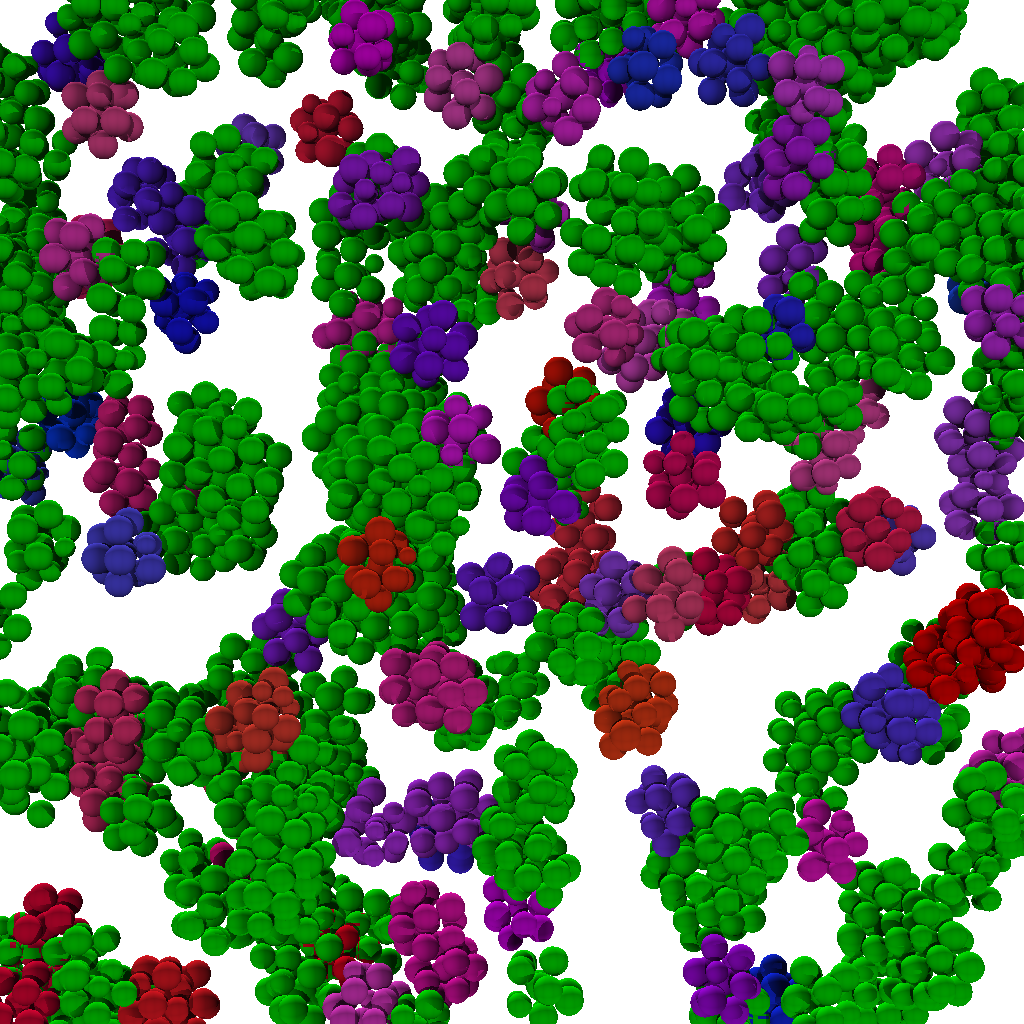
\includegraphics[width=0.6\textwidth]{mrco_ico_scale_go1-0023.png}};
	\matrix[%
		matrix of nodes, ampersand replacement=\&,%
		matrix anchor=east, draw, font=\footnotesize,% 
		column 1/.style={text height=0.8em, text depth=0.2em},%
		column 2/.style={circle, shade, inner sep=0.008\textwidth},%
		] (l)
	{
		Icosahedra \& \node[ball color=red!50!blue] (b2) {};\node[ball color=red!75!black, left] at (b2.west) {}; \node[ball color=blue!75!black, right] at (b2.east) {};\\
		Crystal-like \& |[ball color=green!66!black]|\\
	};
	\node[above=0.01\textwidth of l, pic3d, label={\footnotesize $w_6=w_6^*$}, label=left:{local}] (one_ico) {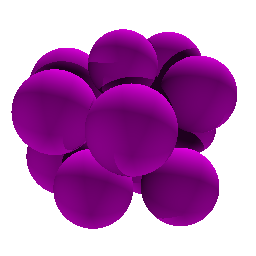
\includegraphics[width=0.2\textwidth]{one_ico.png}};
	\node[below=0.01\textwidth of l, pic3d, label=below:{\footnotesize $Q_6=Q_6^*$}, label={[text width=0.11\textwidth]left:{medium-ranged}}] (one_mrco) {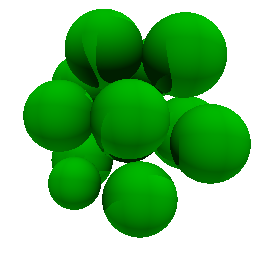
\includegraphics[width=0.2\textwidth]{one_mrco.png}};
	\end{tikzpicture}
\end{frame}

\begin{frame}{Crystal-like order is not crystal}
	\begin{center}
	\begin{columns}
	\column{0.45\textwidth}
	Crystal-like\\
	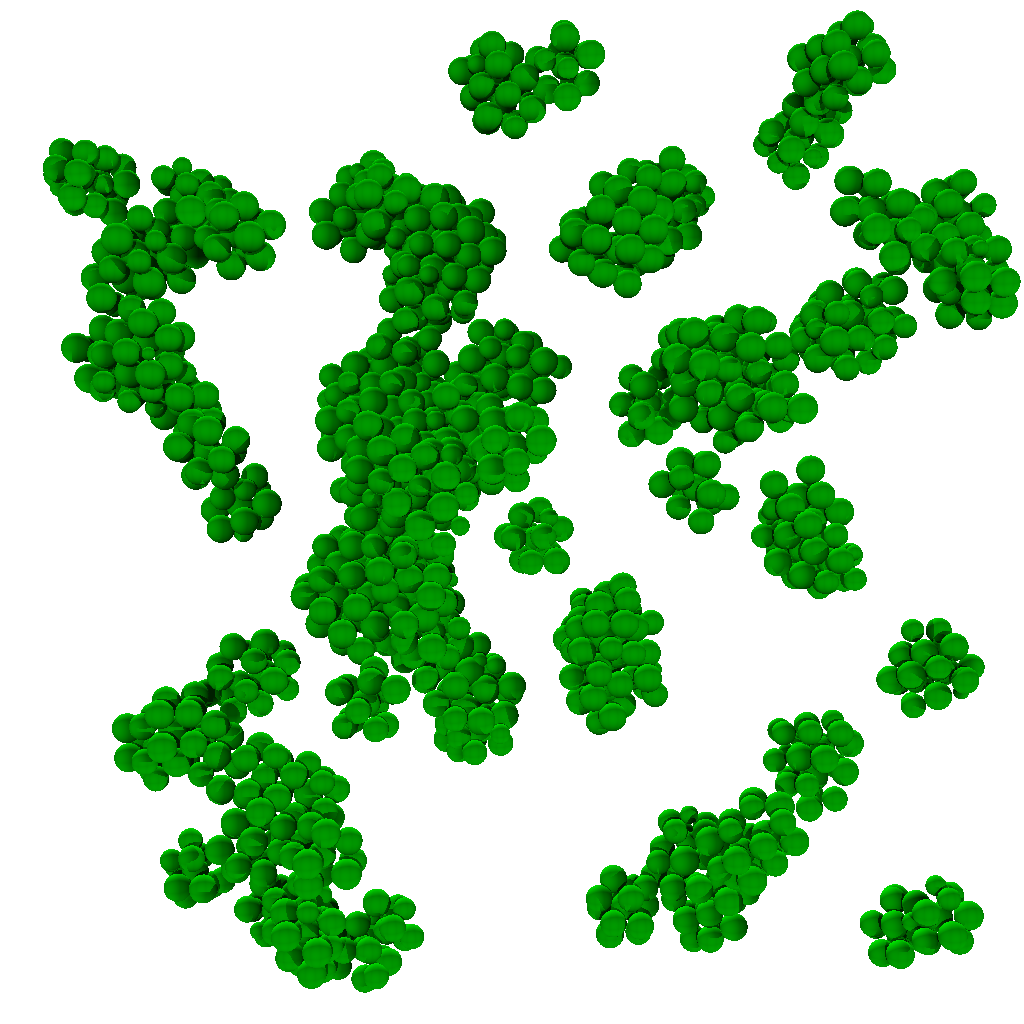
\includegraphics[width=\textwidth]{mrco24_scale_go1_t040_t048.png} 
	\column{0.1\textwidth}
	{\Large $\neq$}
	\column{0.45\textwidth}
	Crystal (Frenkel criteria)
	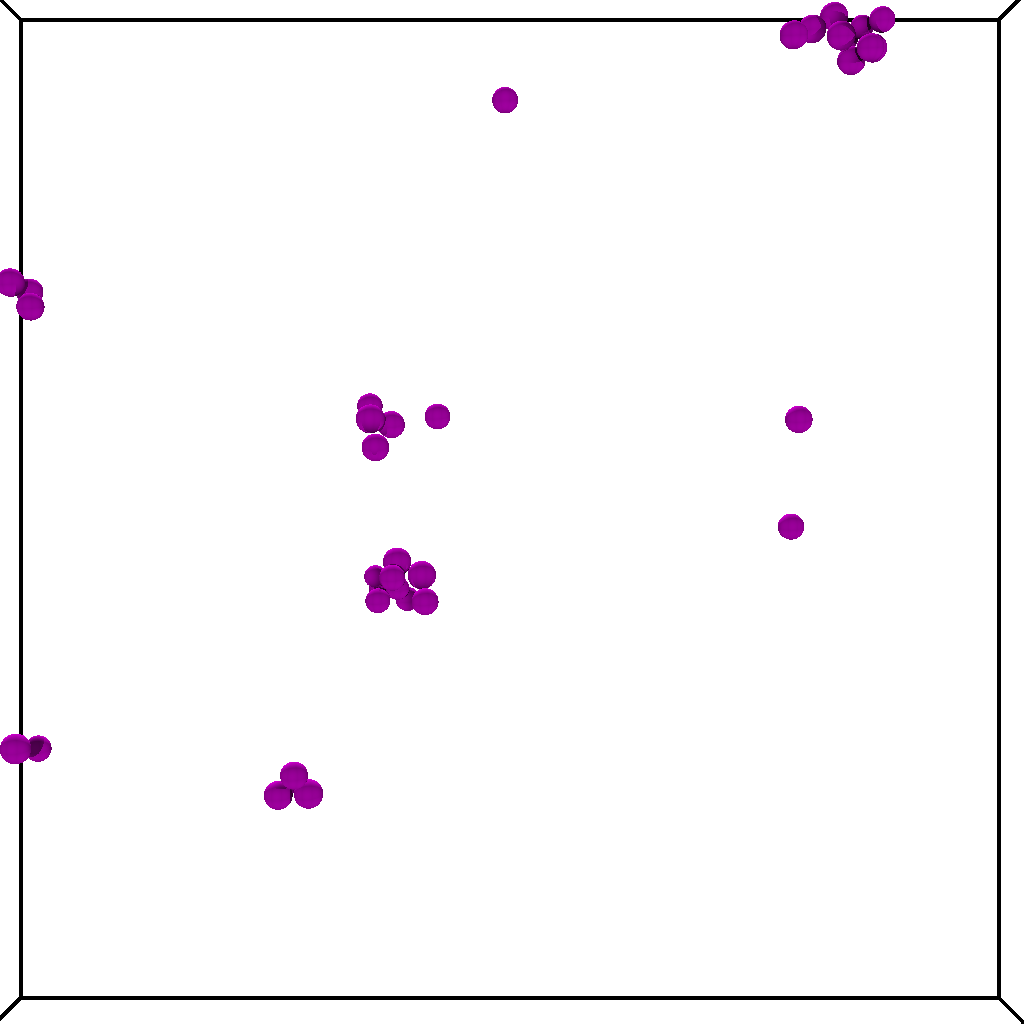
\includegraphics[width=\textwidth]{X_go1.png}
	\end{columns}
	\end{center}
\end{frame}


\begin{frame}{Growing correlation lengths}
	\begin{textblock*}{0.6\textwidth}(10mm,88mm)
		\simplephasediagram{}
	\end{textblock*}
	\begin{columns}
	\column{0.5\textwidth}\centering
	\tikzsetnextfilename{lengths}%
	\begin{tikzpicture}
		\pgfplotsset{cycle list name=black white}
		\tikzset{every mark/.append style={scale=1.2}}
		\begin{axis}[%
			width=\textwidth, %
			xlabel=$\phi$, xmin=0.49, xmax=0.58, xlabel near ticks,%
			xtick={0.5,0.52,...,0.6},%
			ylabel=$\xi/\xi_0$, ymax=10,
			ytick={2,4,6,8},
			ylabel near ticks,%
			label style={font=\tiny}, %
			legend pos=north west,%
			]
			\addplot+[only marks, mark=*, %
				every mark/.append style={fill=black, scale=1.2},
				error bars/.cd, y dir=both, y explicit relative,%
				] table[x index=0, y expr=\thisrowno{3}/0.126]{scale.xi};
			\addplot+[mark=none, forget plot, domain=0.49:0.58] {(0.6/x-1)^(-2.0/3.0)};
			\addplot+[only marks, mark=square, every mark/.append style={draw=gray, scale=1.2},] table[x index=0, y expr=\thisrowno{5}/0.216]{scale.xi};
			\legend{$\xi_u$ dynamical, $\xi_6$ crystal-like};
		\end{axis}
	\end{tikzpicture}
	\column{0.5\textwidth}
	{\footnotesize see also~\citet{tanaka2010critical,Kawasaki2010}}
	
	\bigskip
	
	
	Power-law fit
	\[ \xi(\phi) \propto \xi_0 \left( \frac{\phi_0 - \phi}{\phi} \right)^{-\frac{2}{3}} \]
	\end{columns}
	\begin{itemize}
		\item $\phi_0$ comes from the divergence of $\tau_\alpha$
		\item $\xi_0$ is the only adjustable parameter
		\item Exponent compatible with the Ising universality class
	\end{itemize}
	The divergence of the dynamics is linked to the crystal-like order
\end{frame}

\tikzsetnextfilename{mrco_slow}
\begin{frame}{Crystal-like order governs slow dynamics}
	\begin{tikzpicture}[%
		pic3d/.style={inner sep=0}, %
		]%
	\definecolor{turquoise}{rgb}{0.678431,0.917647,0.917647}
	\node[below=0.01\textwidth, pic3d, label={Slow}] (dyn) {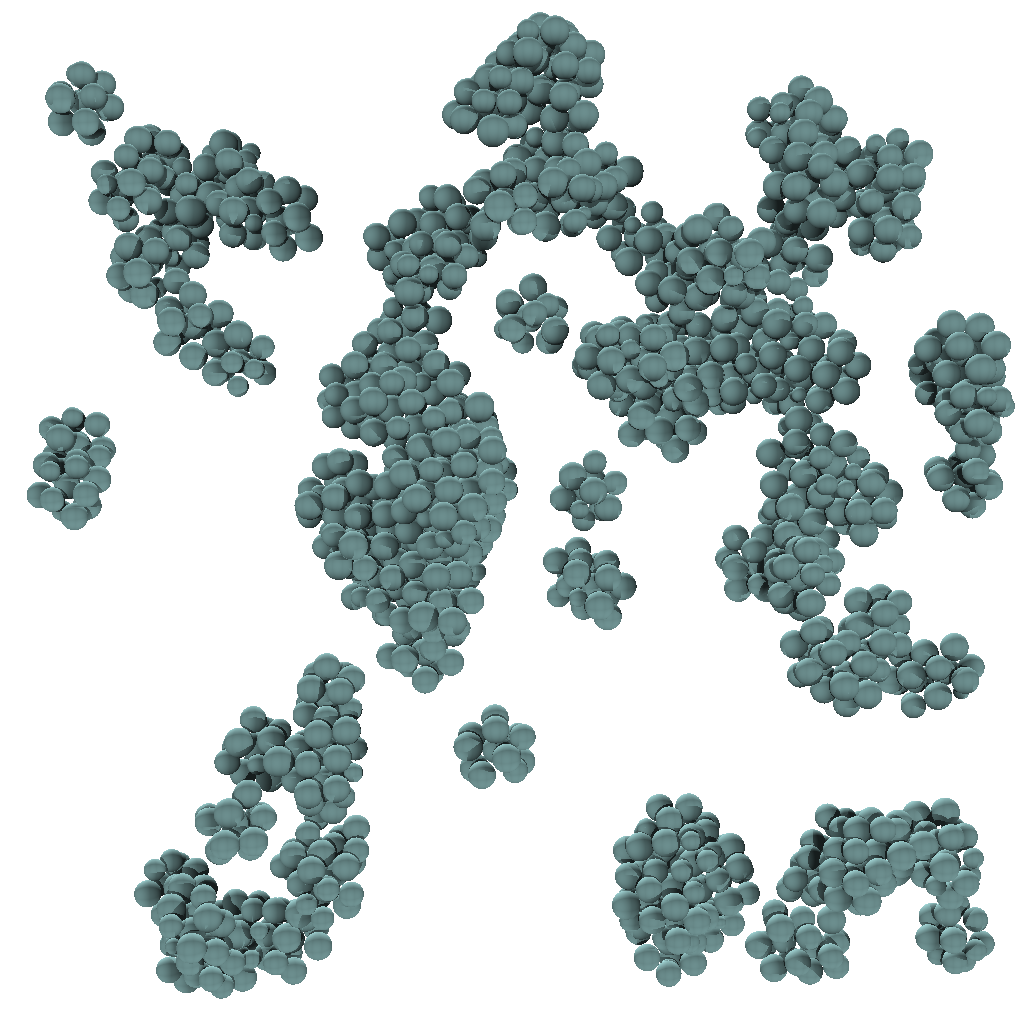
\includegraphics[width=0.48\textwidth]{cgsd_2tau.png}};
	\node[left=0.01\textwidth of dyn, pic3d, label={Crystal-like}] (mrco) {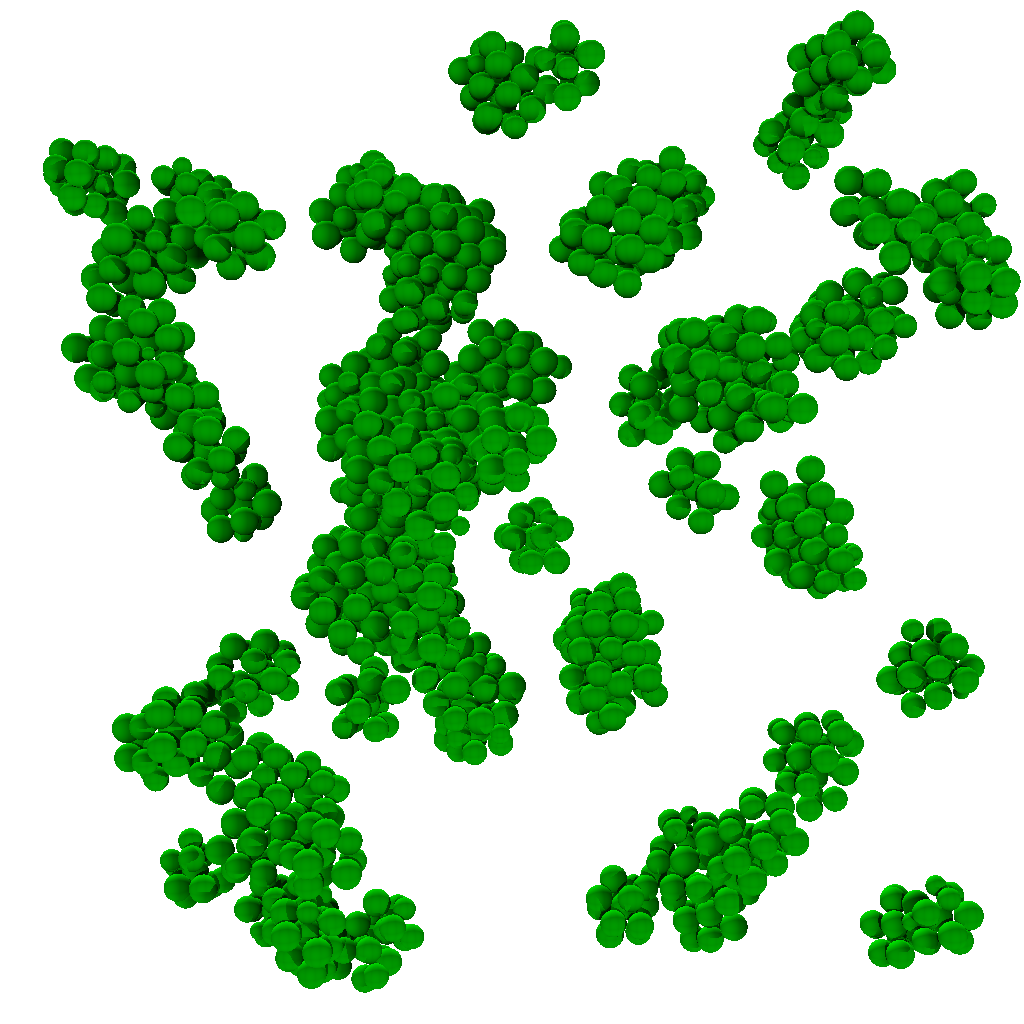
\includegraphics[width=0.48\textwidth]{mrco24_scale_go1_t040_t048.png}};
	\draw [help lines, step=0.12\textwidth, shift=(mrco.south west)] (0, 0) grid (0.48\textwidth, 0.48\textwidth);
	\draw [help lines, step=0.12\textwidth, shift=(dyn.south west)] (0, 0) grid (0.48\textwidth, 0.48\textwidth);
	\node[below=0.01\textwidth of dyn, text width=0.4\textwidth, font=\footnotesize] {$10\%$ shorter displacements after $2\tau_\alpha\approx 4.5 t^{dh}$};
	\node[below=0.01\textwidth of mrco, text width=0.4\textwidth, font=\footnotesize] {$10\%$ higher $Q_6$ (time-averaged over $t^{dh}/2$)};
	\end{tikzpicture}
\end{frame}

\begin{frame}{Icosahedral order role in dynamic heterogeneity}
	\begin{block}{Icosahedral order has}
	\begin{itemize}
		\item No growing length scale
		\item No meaningful percolation
		\item No medium range size
		\item No spatial correlation
	\end{itemize}
	
	\bigskip	
	
	\alert{$\Rightarrow$ no direct role} in the slowing down of the dynamics
	\end{block}
	But probably a frustration role on the crystallisation.
	\begin{itemize}
		\item allows supercooling
		\item linked to the fragility
	\end{itemize}
\end{frame}

\begin{frame}{``Ordered'' particles, various definitions}
\centering
\begin{tabular}{c|c|c}
	Two-body & Icosahedral & Crystal-like\\
	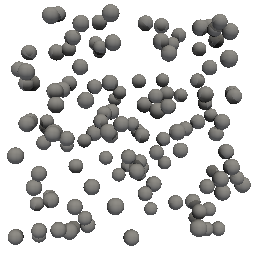
\includegraphics[width=0.25\columnwidth]{s2_slice_3D}&%
	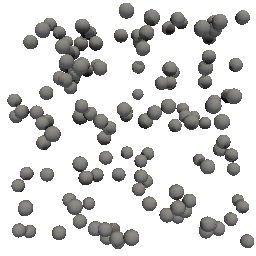
\includegraphics[width=0.25\columnwidth]{q6_slice_3D}&%
	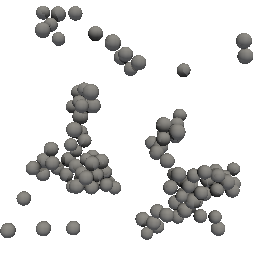
\includegraphics[width=0.25\columnwidth]{Q6_slice_3D}\\ 
	$s_2$ & $q_6$ & $Q_6$ \\ 
	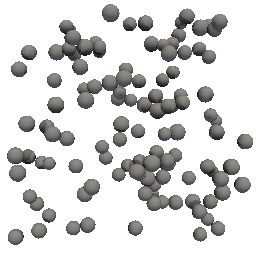
\includegraphics[width=0.25\columnwidth]{f2_slice_3D}&%
	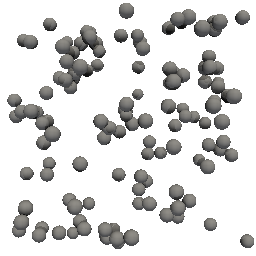
\includegraphics[width=0.25\columnwidth]{w6_slice_3D}&%
	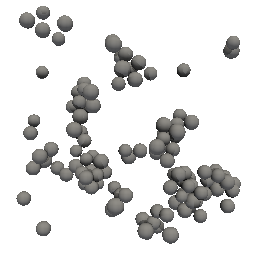
\includegraphics[width=0.25\columnwidth]{C_slice_3D}\\ 
	$f_2$ & $w_6$ & $C$ \\ 
\end{tabular}

{\footnotesize Leocmach, Russo, \& Tanaka \textit{J. Chem. Phys.} 138, 12A536 (2013)}
\end{frame}

\begin{frame}{Length scales}
	\tikzsetnextfilename{two_body_multi_body_lengths}%
	\begin{tikzpicture}
	\pgfplotsset{every axis/.append style={
		height=0.6\columnwidth,%
		width=0.95\columnwidth,
		cycle list name=exotic,
		xlabel={Pressure},
		ymin=0,
		xmin=8,
		xtick={9,13,...,25},
	}}
	\begin{axis}[%
		name=len,
		ylabel={Correlation length},
		ymax=1.6,
		legend style={at={(1,1.03)}, anchor=south east},
		legend columns=10,
		]
	\pgfplotstableread{lengths}\lengths
	 \foreach \y in {1, 2, ..., 6} {
          \addplot table[x index=0, y index=\y]{\lengths};
          \pgfplotstablegetcolumnnamebyindex{\y}\of{\lengths}\to{\colname}
          \addlegendentryexpanded{$\colname$}
          }
	\end{axis}
	\end{tikzpicture}
\end{frame}